\documentclass[tikz]{standalone}

\usetikzlibrary{intersections, angles}

\begin{document}
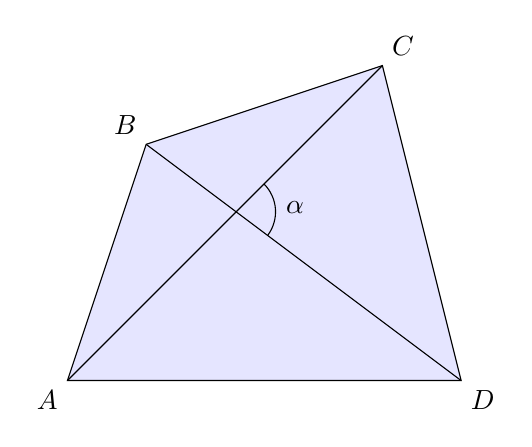
\begin{tikzpicture}

\coordinate (A) at (0, 0);
\coordinate (B) at (1, 3);
\coordinate (C) at (4, 4);
\coordinate (D) at (5, 0);
\draw[fill=blue!10!white]
    (A) node[below left]{$A$}
    -- (B) node[above left]{$B$}
    -- (C) node[above right]{$C$}
    -- (D) node[below right]{$D$}
    -- cycle;

\draw [name path=diagAC] (A) -- (C);
\draw [name path=diagBD] (B) -- (D);

\path [name intersections={of=diagAC and diagBD, by=P}];
\pic [draw, pic text = $\alpha$, angle eccentricity=1.5] {angle = D--P--C};

\end{tikzpicture}
\end{document}
